\chapter{planning}

This chapter presents the work plan to follow to carry out this study. First of all, the requirements necessary to achieve the proposed objective will be captured, and then the work planning will be detailed, with an estimate of both work and material costs as well as a distribution of time between tasks.

\section{Investigation stages}
The steps of the research process of this study are as follows:

\begin{enumerate}
    \item{\textbf{Initiate a preliminary investigation of the Cryptanalysis:} review many of theses and papers looking for information about Cryptanalysis, check what evolution they have followed over the years and how the Cryptanalysis systems have been developed.}
    \item{\textbf{delve into the Transposition and Substitution ciphers:} investigate further in these types that are really going to focus on the study}
    \item {\textbf{Select the algorithm:} investigated in the previous steps, deciding the most appropriate option.}
    \item {\textbf{delve into genetic algorithm:} Study and understand all stages of genetic algorithm evolution and how to solve current problems, review the papers that related with GA.}
    \item {\textbf{Implement genetic algorithm:} create a set of classes, each of them performs stage of GA stages and all of them has a set of methods to divide its stage to small tasks every task solves a different problem.}
    \item {\textbf{create a new proposal for the study:} for the objective of the study, new proposals that can compete with the state of the art must be proposed.}
    \item {\textbf{Implement my new proposal:} that will be part of the experiment have been decided, they must be implemented in the same way as the state of the art algorithm. Check of new that all the functionality of the experiment is valid with the new implementation.}
    \item {\textbf{Obtain the results of the experiment:} obtain through the implementation of the experiment, can visualize the data in tables and graphs that are suitable for the study.}
    \item {\textbf{analysis of the results obtained:} compare the results of each method with the \textit{baseline} reference method and with the state of the art method, as well as between them, to discover which method behaves best for each case.}
    \item {\textbf{Consider future work to be done:} assess the aspects it is possible to continue progressing in the methods proposed in the study, propose new tasks or challenges within this field of research, that have not been covered in this study.}
\end{enumerate}

\section{Work plan}
This section is subdivided into cost estimation and time estimation. In the first place, The cost of the infrastructure used is evaluated, as long as the material that has been used is available for free and free. From there we can make a base budget from which to start. The time estimate should be realistic and meet the requirements within a competent time frame so that you do not need to postpone times at the last minute due to poor planning. If so, it would be necessary to bear the consequent increase in costs.
\subsection{Cost estimate of materials and infrastructure}
First of all, the computer with which this study has been developed will be taken, the following hardware and software have been used for this study:
\textbf{Computer Type:}Lenovo IdeaPad Z510.
\textbf{Processor:}Intel(R) Core(TM) i7-4702MQ CPU@ 2.20GHz 2.20GHz.
\textbf{Installed memory (RAM):} 8.00 GB.
\textbf{graphics card:} Intel(R) HD Graphics 4600, Memory:2176 MB.
\textbf{Hard Disk:} HDD 1TB

\textbf{Operating system:} Win10.
\textbf{Programming language:} java.
\textbf{Environment:}  NetBeans 8.1.
All the research, implementation, and evaluation tasks have been carried out with this team: documentation, review of the literature, writing of the report, development, implementation of the algorithms, and execution of the experiment to obtain results.

information and documentation required for the work are available  at the University of Granada  Thanks to the agreements that the University establishes with some documentary databases such as Scopus, it has been possible to access a multitude of papers and theses on the subject to be investigated. Furthermore, the Google scholer has been very useful to access other papers not found in Scopus.

The development of the work has been carried out entirely on the Win10 OS, The main software tools used have been open source so they have not entailed additional cost, Netbeans as the main IDE for development and writing the report of the project in LaTeX using the TeXstudio, available for win 10, and  we used  Visual Studio Code as an IDE to deal with the repository of the project that has hosted on \textbf{GitHub} \cite{MyProject} platform, and we used \textbf{Travis CI} \cite{travis_CI} to host continuous integration service used to build and test software projects hosted at GitHub,Travis CI provides various paid plan for private projects, and a free plan for open source.
Of all this material exposed in the previous paragraphs, the work has only required buying the personal laptop and the broadband network available, The rest of the infrastructure and materials have either been free software products or have been contributed by the University of Granada.

\subsection{Time distribution to the tasks}
we used the concepts of iterations and sprints to distribute the work throughout the weeks, in which a series of tasks have been developed that they fulfill a specific objective.

The Iteration and Sprint Planning meeting is for team members to plan and agree on the stories or backlog items they are confident they can complete during the sprint and identify the detailed tasks and tests for delivery and acceptance

The planning that has been foreseen for the development of the project is as follows:

\begin{table}[h!]
    \centering
    \begin{tabular}{|p{5cm}|p{4cm}|}
     \hline
        \cellcolor[gray]{0.9} Weeks  & 10 \\ \hline
        \cellcolor[gray]{0.9} Estimated total time (h)  & 240h \\ \hline
        \cellcolor[gray]{0.9} date of Starting Point  & 01-06-2020 \\ \hline
        \cellcolor[gray]{0.9} date of end Point   & 10-09-2020 \\ \hline
            
    \end{tabular}
    \end{table}

\subsection{Preparatory phase}
In this phase, the development of the project will begin, which has an estimated effort of 40 hours. A feasibility study of the project idea will be carried out, an investigation about the possible tools to use


\large{\underline{\textbf{Iteration 1}: Analysis and study of the project.}}
\vspace{0.3cm}
\begin{table}[h!]
    \centering
    \begin{tabular}{|p{5cm}|p{4cm}|}
     \hline
        \cellcolor[gray]{0.9} week  & 1\\ \hline
        \cellcolor[gray]{0.9} Total expected time (h)  & 40h \\ \hline
        \cellcolor[gray]{0.9} date of Starting Point  & 01-06-2020 \\ \hline
        \cellcolor[gray]{0.9} date of end Point  & 06-06-2020 \\ \hline
            
\end{tabular}
\end{table}

\textbf{Sprint 1}: Description of the Project

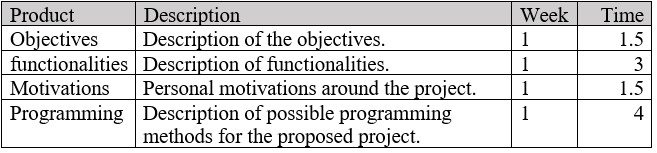
\includegraphics[width=0.9\textwidth]{imagenes/it1sp1.png}\\[1.4cm]
\textbf{Sprint 2}: Research and preparation of the environment.

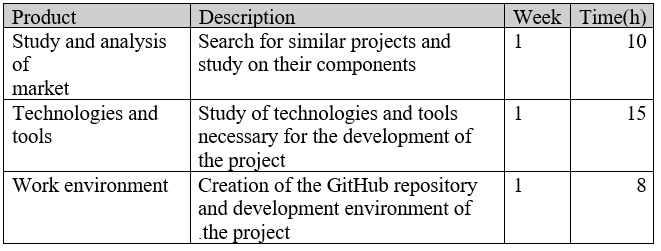
\includegraphics[width=0.9\textwidth]{imagenes/it1sp2.png}\\[1.4cm]

\subsection{Implementation and testing phase}

the objective of this phase is getting an general idea of this project and at the end of this phase, a software-implemented incrementally have been obtained, where each module has been tested until integration and validation.
A total of 280 hours has been planned for this phase, and it has been distributed in the following iterations:

\large{\underline{\textbf{Iteration 2}: Implementation of the main classes.}}
\vspace{0.3cm}

The objective of this iteration is the implementation of the main classes  which will create the system,For this operation, the following schedule has been established:

\begin{table}[h!]
    \centering
    \begin{tabular}{|p{5cm}|p{4cm}|}
     \hline
        \cellcolor[gray]{0.9} week  & 6\\ \hline
        \cellcolor[gray]{0.9} Total expected time (h)  & 120h \\ \hline
        \cellcolor[gray]{0.9} date of Starting Point  & 07-06-2020 \\ \hline
        \cellcolor[gray]{0.9} date of end Point  & 18-07-2020 \\ \hline
            
\end{tabular}
\end{table}

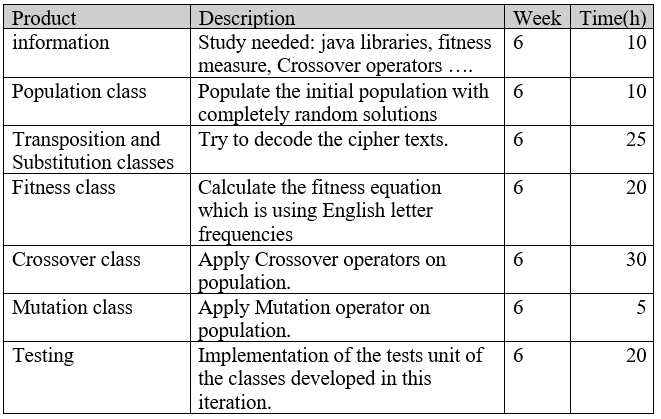
\includegraphics[width=0.9\textwidth]{imagenes/it2.png}\\[1.4cm]

\large{\underline{\textbf{Iteration 3}: Experimental results and Improvement.}}
\vspace{0.3cm}
The objective of this iteration is trying to get a result from the classes then try to improve all of them to get better results,For this iteration, the following schedule has been established:

\begin{table}[h!]
    \centering
    \begin{tabular}{|p{5cm}|p{4cm}|}
     \hline
        \cellcolor[gray]{0.9} week  & 10\\ \hline
        \cellcolor[gray]{0.9} Total expected time (h)  & 120h \\ \hline
        \cellcolor[gray]{0.9} date of Starting Point  & 18-07-2020 \\ \hline
        \cellcolor[gray]{0.9} date of end Point  & 18-08-2020 \\ \hline
            
\end{tabular}
\end{table}

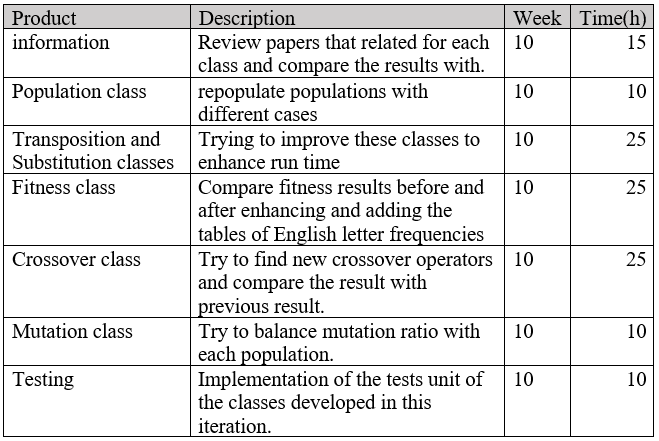
\includegraphics[width=0.9\textwidth]{imagenes/it3.png}\\[1.4cm]

\subsection{Documentation phase}
After the project is completed and approved, it is time to document all of the steps and how to work, and document the achieving result.

the documentations have been divided into two parts. The first one corresponds to the documentation in the Github repository. This documentation has as objective to give an idea about the project in general then delve in details until arrives in programming steps that explain all of the class and their methods and variables,  Anyone who accesses to the repository, he can see all this information as a free software project.

Other documents made are those for the project. In this case, more documentation focused on the scope of the project will be implemented: planning, research, development, Conclusions.
\newpage
\large{\underline{\textbf{Iteration 4}: GitHub Documentation.}}
In this phase has an estimated effort of 50 hours.

\begin{table}[h!]
    \centering
    \begin{tabular}{|p{5cm}|p{4cm}|}
     \hline
        \cellcolor[gray]{0.9} week  & 11\\ \hline
        \cellcolor[gray]{0.9} Total expected time (h)  & 50h \\ \hline
        \cellcolor[gray]{0.9} date of Starting Point  & 18-08-2020 \\ \hline
        \cellcolor[gray]{0.9} date of end Point  & 24-08-2020 \\ \hline
            
\end{tabular}
\end{table}

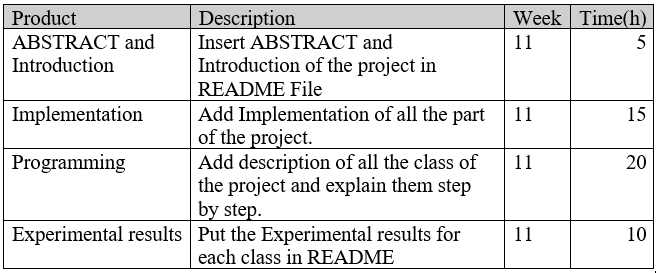
\includegraphics[width=0.9\textwidth]{imagenes/it4.png}\\[1.4cm]

\large{\underline{\textbf{Iteration 5}: Project documentation.}}

In this phase has an estimated effort of 150 hours.

\begin{table}[h!]
    \centering
    \begin{tabular}{|p{5cm}|p{4cm}|}
     \hline
        \cellcolor[gray]{0.9} week  & 13\\ \hline
        \cellcolor[gray]{0.9} Total expected time (h)  & 150h \\ \hline
        \cellcolor[gray]{0.9} date of Starting Point  & 24-08-2020 \\ \hline
        \cellcolor[gray]{0.9} date of end Point  & 09-09-2020 \\ \hline
            
\end{tabular}
\end{table}

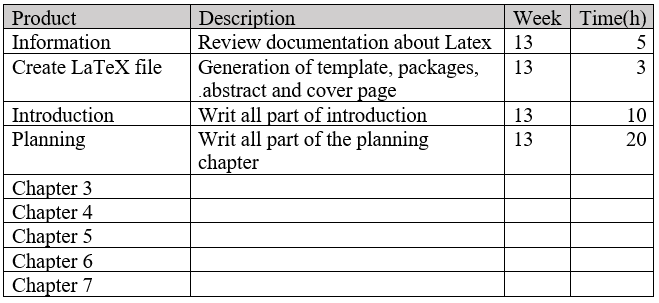
\includegraphics[width=0.9\textwidth]{imagenes/it5.png}\\[1.4cm]
